\documentclass[12pt]{article} % use larger type; default would be 10pt
\usepackage[utf8]{inputenc} % set input encoding (not needed with XeLaTeX)

%%% PAGE DIMENSIONS
\usepackage{geometry} % to change the page dimensions
\geometry{a4paper} % or letterpaper (US) or a5paper or....
\geometry{margin=2cm} % or letterpaper (US) or a5paper or....

\usepackage{graphicx} % support the \includegraphics command and options
\usepackage[parfill]{parskip} % Activate to begin paragraphs with an empty line rather than an indent
\usepackage{times} % for Times Roman default font

%%% PACKAGES
\usepackage{booktabs} % for much better looking tables
\usepackage{array} % for better arrays (eg matrices) in maths
\usepackage{paralist} % very flexible & customisable lists (eg. enumerate/itemize, etc.)
\usepackage{verbatim} % adds environment for commenting out blocks of text & for better verbatim
\usepackage{subfig} % make it possible to include more than one captioned figure/table in a single float
\usepackage{caption}

%%% HEADERS & FOOTERS
\usepackage{fancyhdr} % This should be set AFTER setting up the page geometry
\pagestyle{fancy} % options: empty , plain , fancy
\renewcommand{\headrulewidth}{0pt} % customise the layout...
\lhead{}\chead{}\rhead{}
\lfoot{}\cfoot{\thepage}\rfoot{}

\makeatletter
\renewcommand{\maketitle}{%
  {\bfseries{\scshape{\Large{\@title\par}}}}
}
\makeatother

\hyphenation{Kiwi-bank} % otherwise it may get hyphenated as Ki-wibank

%%% END Article customizations

%%% The "real" document content comes below...

\title{Lake Man Biv Report: April 2019}

\begin{document}
  \maketitle

\begin{figure}[t]
%\centering
\begin{minipage}{.3\linewidth}
\begin{flushleft} 
   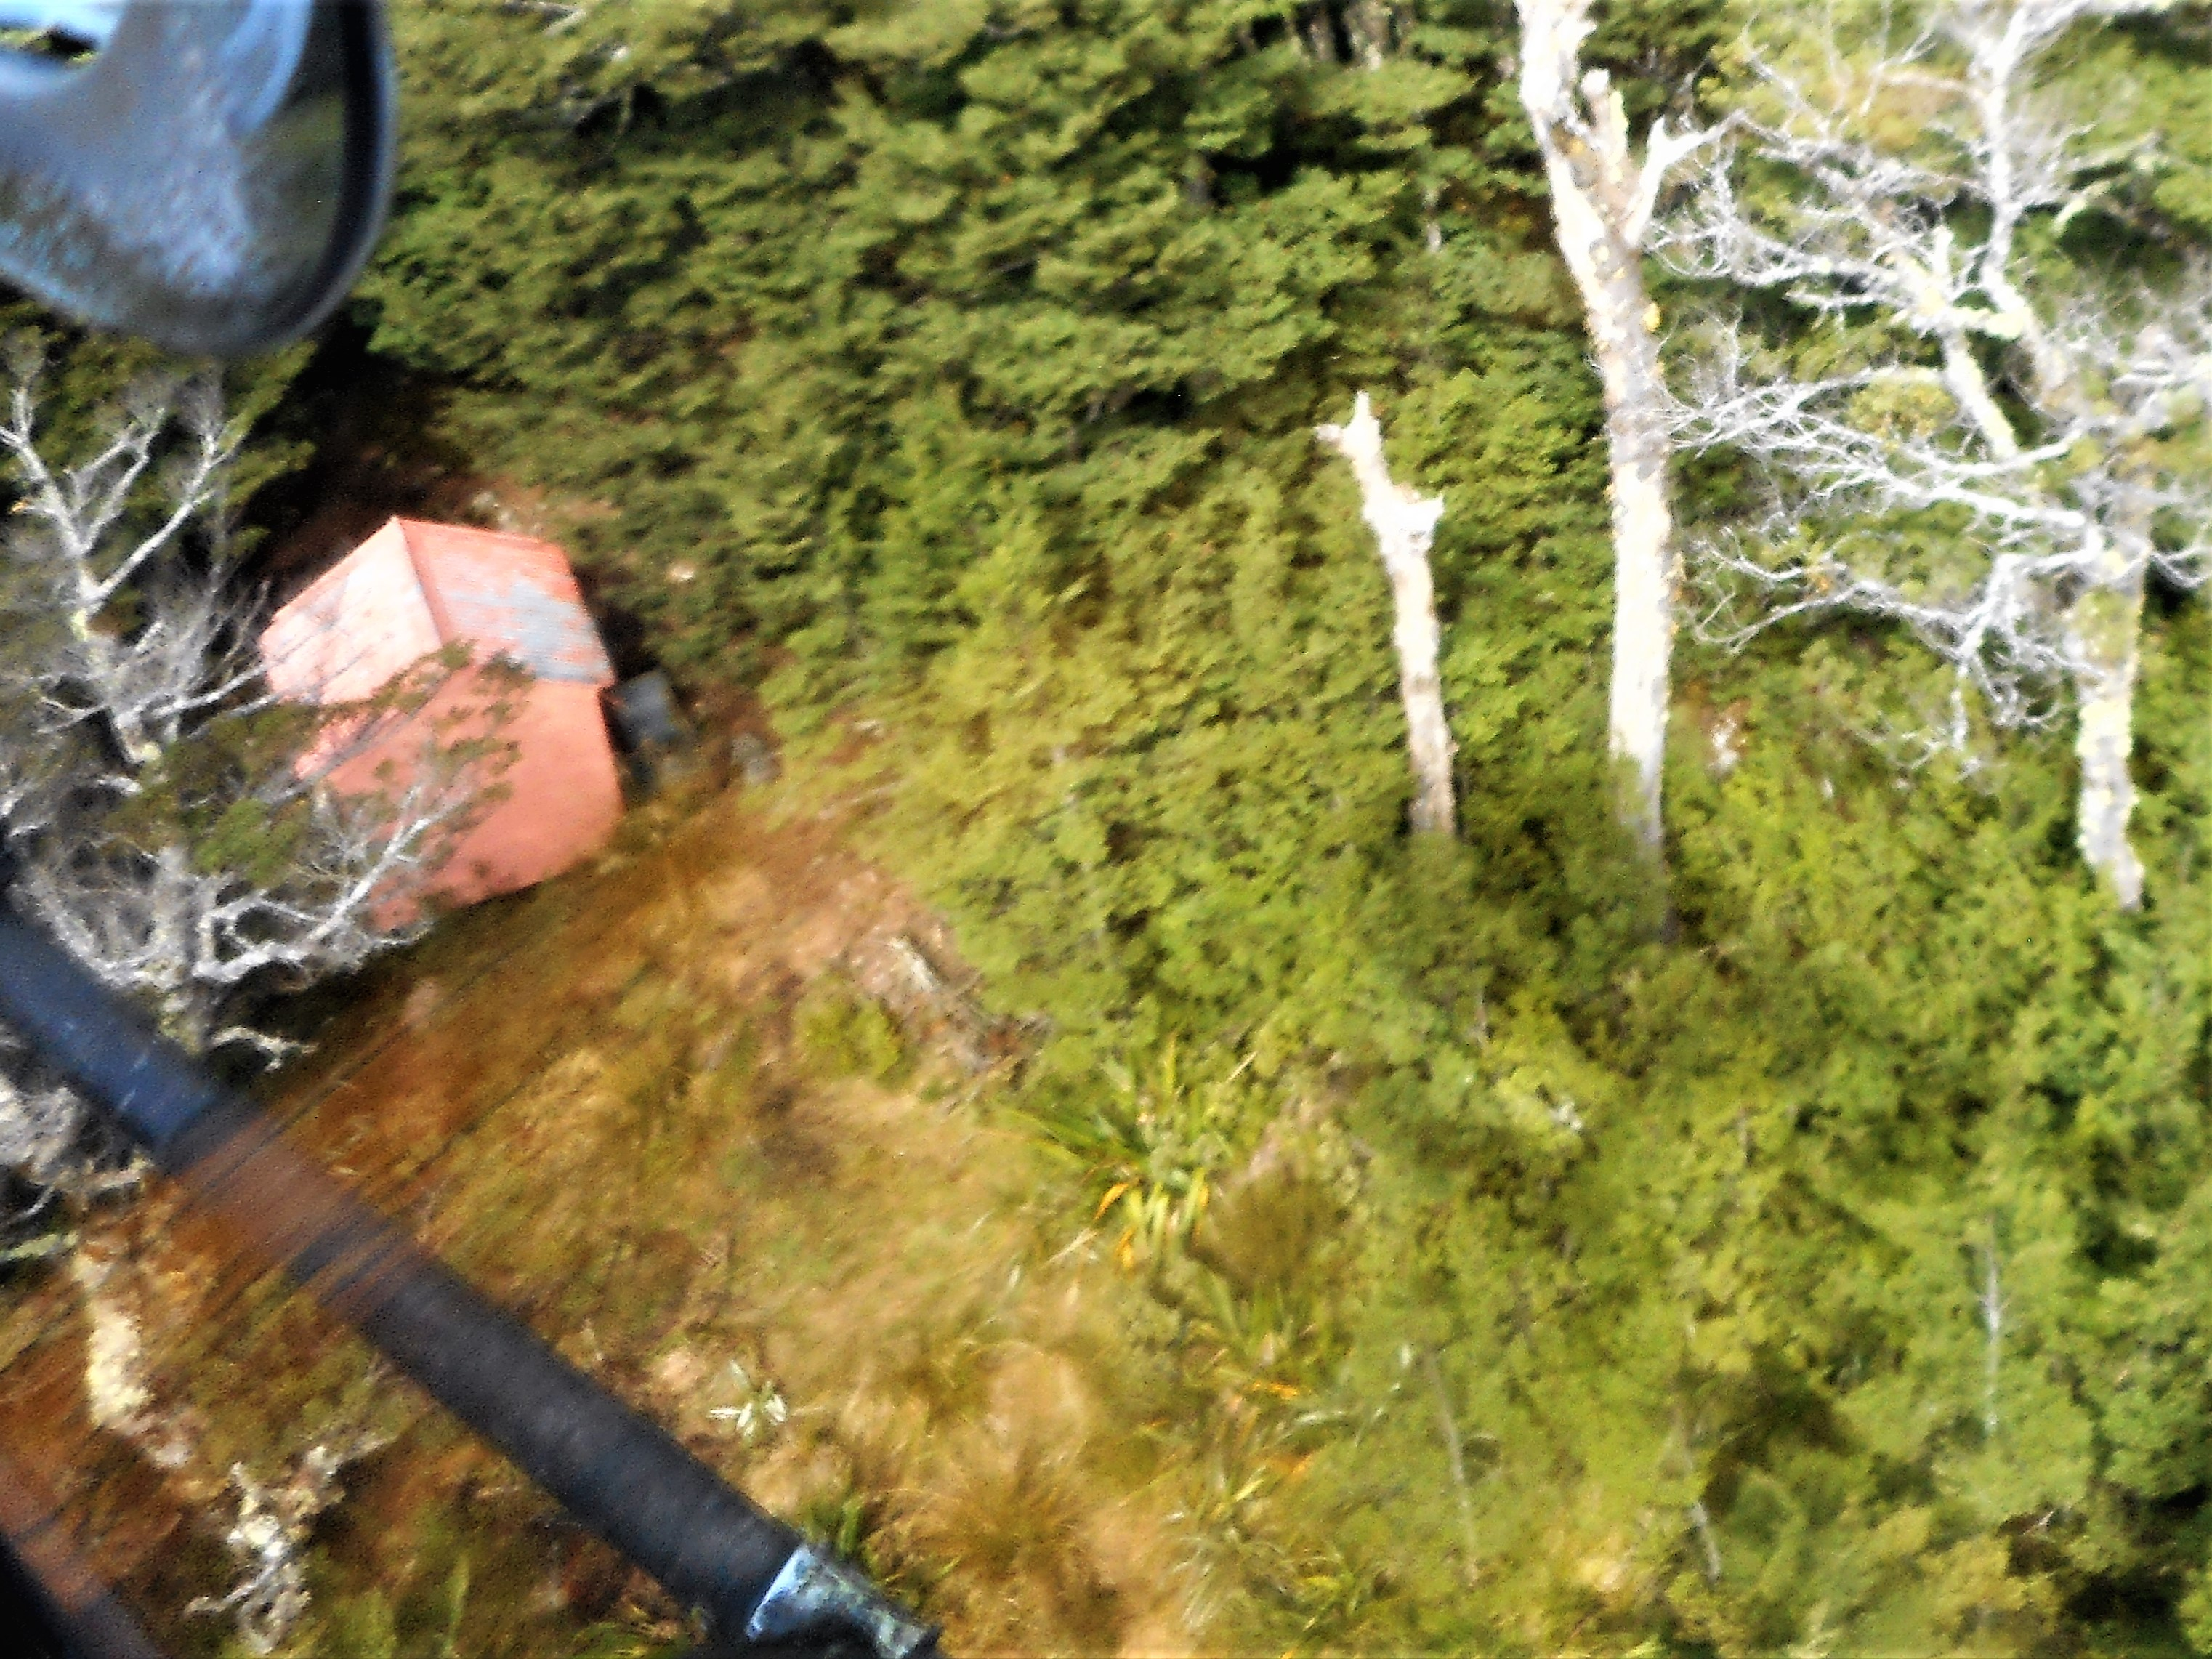
\includegraphics[width=4.5cm]{LakeManBivReportApr2019Photo01}
\end{flushleft} 
\end{minipage}
\begin{minipage}{.3\linewidth}
\begin{center} 
   \includegraphics[width=5.5cm]{LakeManBivReportApr2019Photo03}
\end{center} 
\end{minipage}
\hspace{.05\linewidth}
\begin{minipage}{.3\linewidth}
\begin{flushright} 
    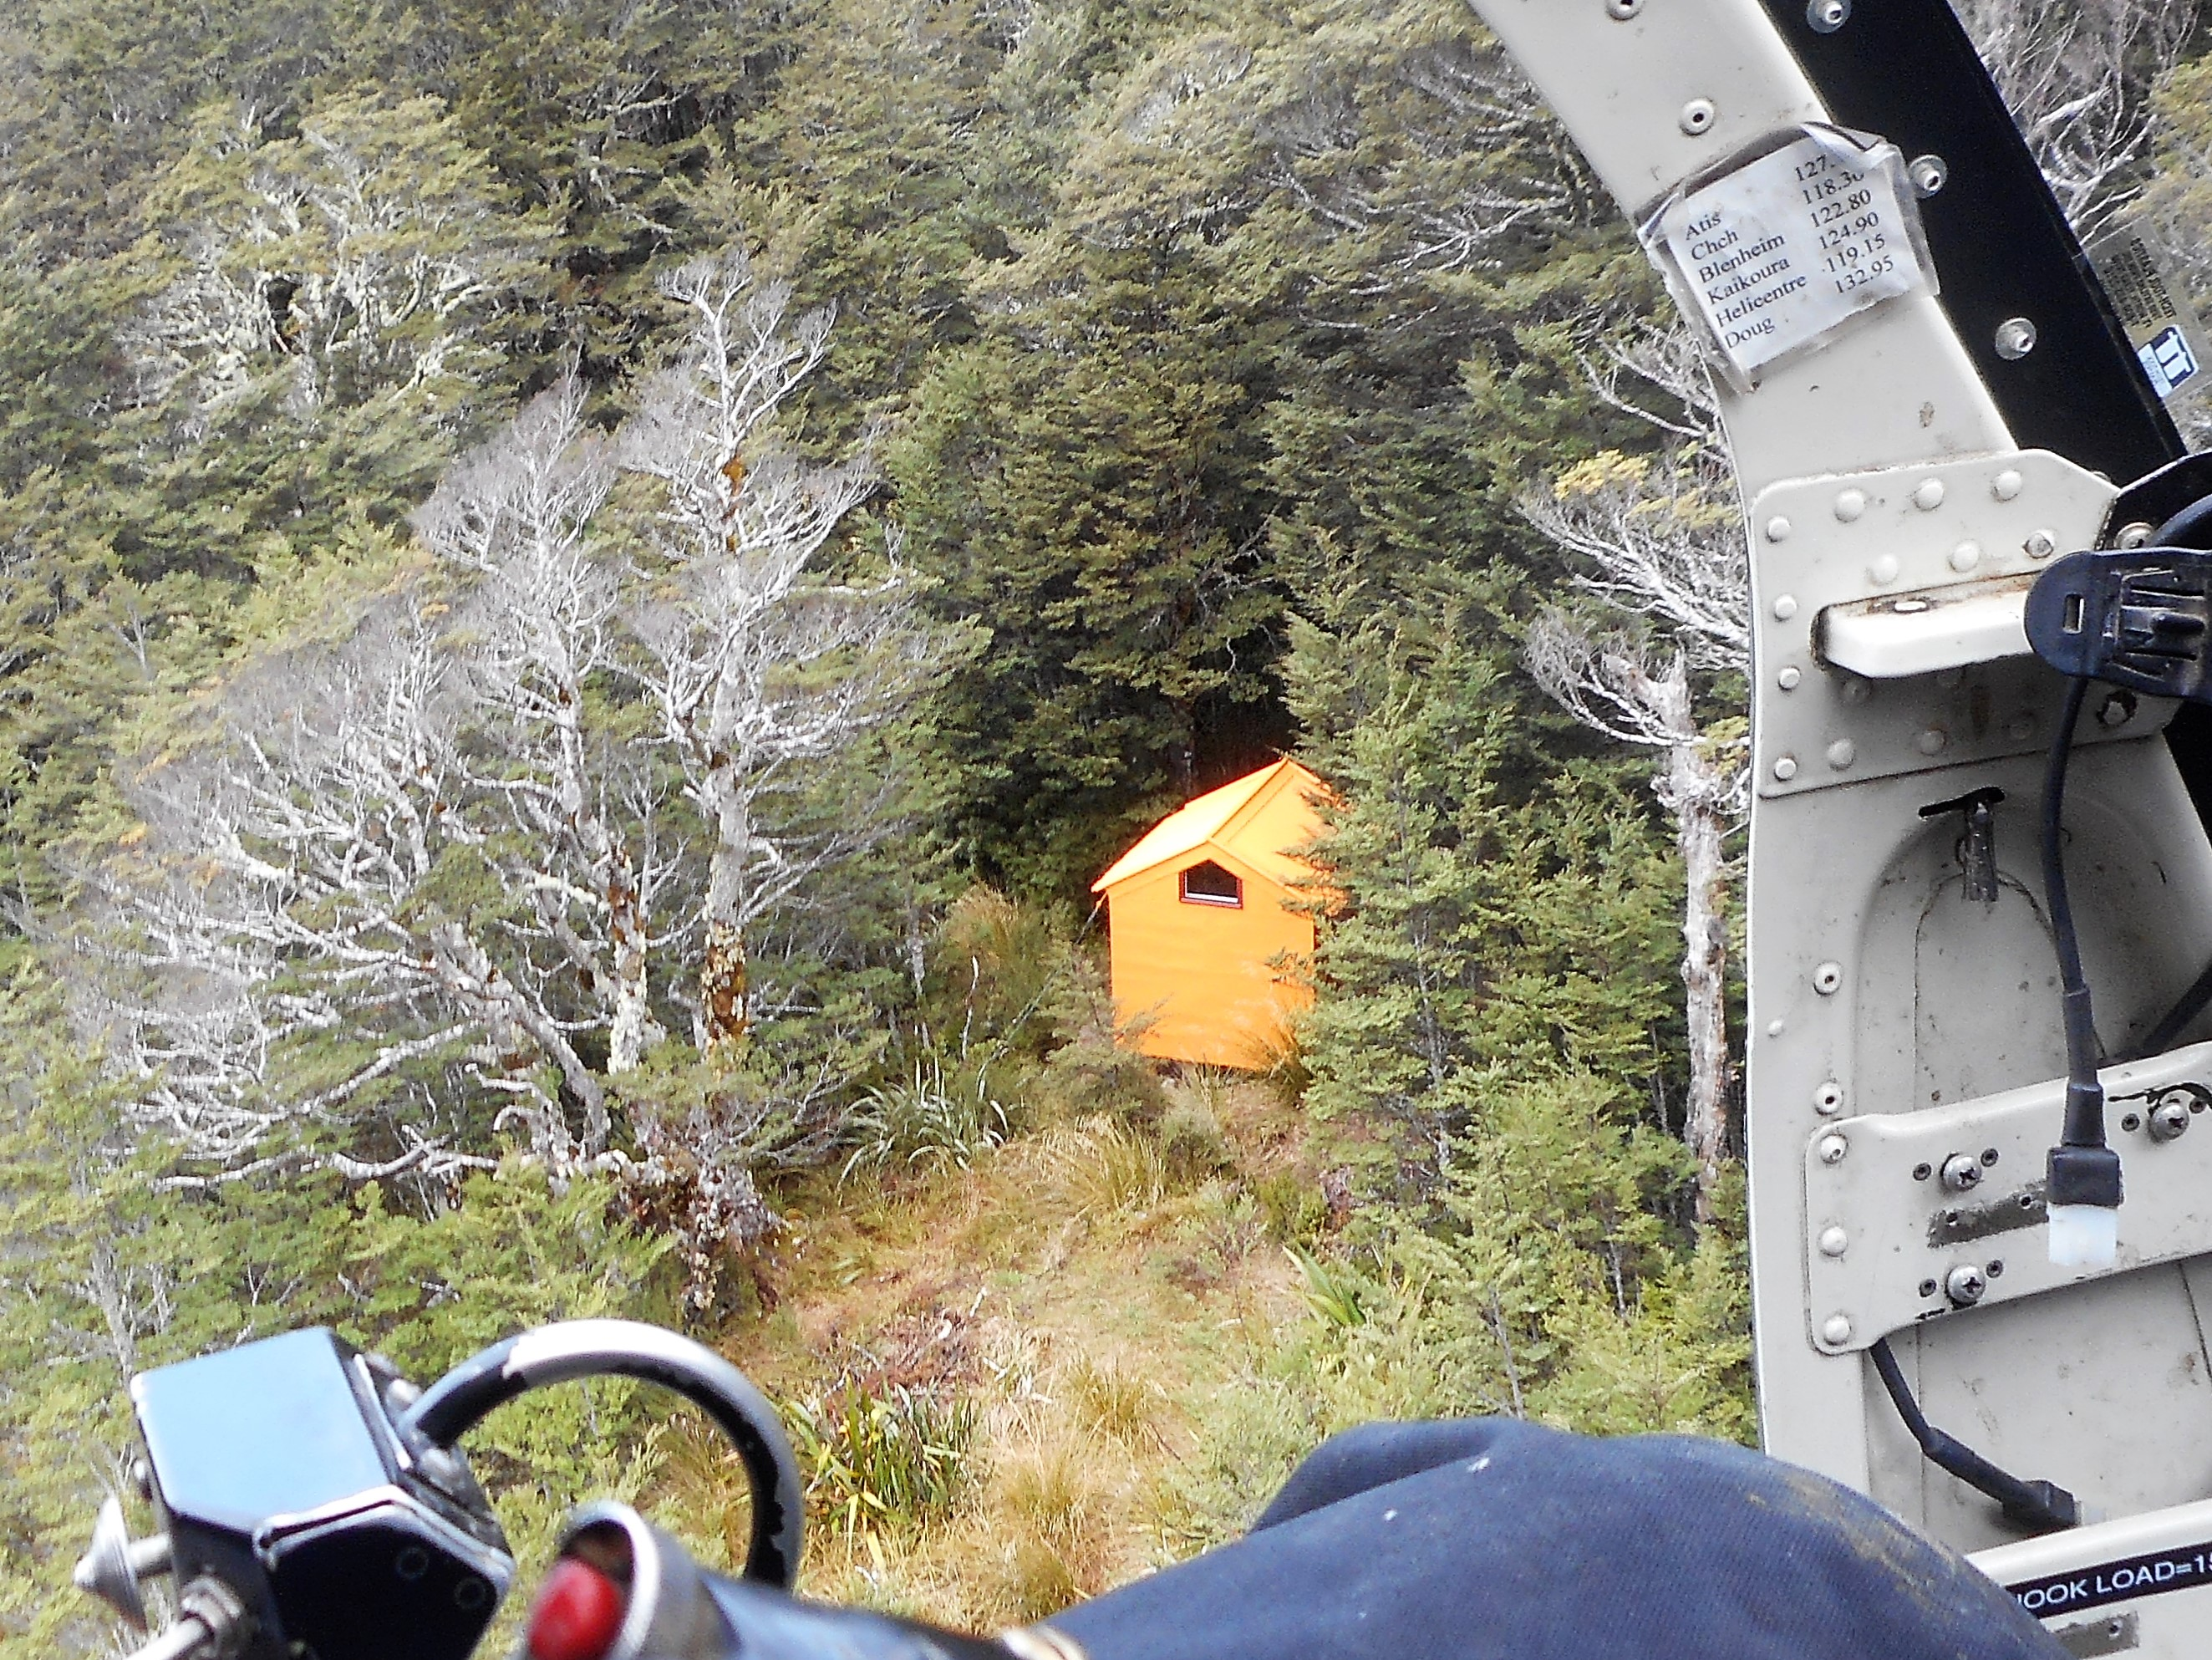
\includegraphics[width=4.5cm]{LakeManBivReportApr2019Photo02}
\end{flushright} 
\end{minipage}
\end{figure}

\section{Background}

On 3 September 2017, we visited Lake Man Biv to assess what needed to be done by way of maintenance and renovation.  On 4 April 2019 we flew in to undertake the work as identified at that time (and confirmed with a more recent visit in January 2019).  This report documents what was achieved before we flew out late afternoon on 9 April.

\section{Maintenance and renovation}

\subsection{Required work}

\subsubsection{Done}

\begin{itemize}
 \item Replaced the lead-head nails with hex-screws.  The ridge cap still has lead edging but this has been well painted, and is (hopefully) unlikely to attract the attention of kea
 \item Filled a few small nail holes in the cladding
 \item Painted the exterior:
 \begin{itemize}
  \item Preparation: It rained (and snowed) on 5-7 April, and the temperature never reached 10$^{\circ}$C.  On these three days the exterior was prepared for painting.  On the roof, most existing paint was removed (Figure \ref{LMB4})
  \item On the morning of 8 April the Biv was fully primed (Figure \ref{LMB6})
  \item The first top coat was applied in the afternoon, and the second the following day (Figure \ref{LMB7})
 \end{itemize}
 \item Dug a trench on the upper (i.e., south) side of the Biv (Figure \ref{LMB4}).  This will need regular clearing
 \item Removed some accumulated rubbish
 \item A pick-axe was left for digging toilet holes
\end{itemize}

\subsubsection{Not done}
\begin{itemize}
 \item A weather ledge on the exterior of the door was not fitted
\end{itemize}

\begin{figure}[ht]
%\centering
\begin{minipage}{.5\linewidth}
\begin{flushleft}
  \includegraphics[width=8cm]{LakeManBivReportApr2019Photo04}
  \caption{Roof ready for painting}
  \label{LMB4}
\end{flushleft}
\end{minipage}
\begin{minipage}{.5\linewidth}
\begin{center}
  \includegraphics[width=8cm]{LakeManBivReportApr2019Photo06}
  \caption{Fully primed}
  \label{LMB6}
\end{center}
\end{minipage}
\end{figure}

\begin{figure}[ht]
%\centering
\begin{minipage}{.5\linewidth}
\begin{flushleft}
  \includegraphics[width=8cm]{LakeManBivReportApr2019Photo07}
  \caption{Biv fully painted}
  \label{LMB7}
\end{flushleft}
\end{minipage}
% \begin{minipage}{.5\linewidth}
% \begin{center}
%   \includegraphics[width=8cm]{LakeManBivReportApr2019Photo06}
%   \caption{Fully primed}
%   \label{LMB6}
% \end{center}
% \end{minipage}
\end{figure}

\subsection{Desirable}

\subsubsection{Done}

\begin{itemize}
 \item As the weather precluded the option of removing the roof, the ceiling was insulated from inside and lined with ply under the rafters (Figures \ref{LMB9} and \ref{LMB10}).  This had the advantage of allowing more insulation (about 100mm \textit{cf} about 40mm).  However, it has slightly decreased the internal height of the Biv
 \item Installed internal trim around the doorway to reduce unwanted draft
 \item Fitted an internal door bolt
 \item The bench was replaced with a stainless-steel topped one located under the window (Figure \ref{LMB8}). The existing bench was freed from the floor and left so that it could be used outside when the weather permits (we found this useful)
 \item Rebuilt the shelves (Figure \ref{LMB9}).  These are now much sturdier
 \item Supplied mattresses (Figure \ref{LMB10}).  The canvas was removed and replaced with slats to accommodate the mattresses.  A third mattress was not left as we consider there to be insufficient space
 \item Installed a small double-glazed window in the apex on the west wall\footnote{Mistakenly referred to as the south wall in the September 2017 report.} (Figures \ref{LMB5} and \ref{LMB6})
\end{itemize}

\begin{figure}[ht]
%\centering
\begin{minipage}{.5\linewidth}
\begin{flushleft}
   \includegraphics[width=8cm]{LakeManBivReportApr2019Photo08}
   \caption{New bench under the window}
   \label{LMB8}
\end{flushleft}
\end{minipage}
\begin{minipage}{.5\linewidth}
\begin{center}
   \includegraphics[width=8cm, angle=270]{LakeManBivReportApr2019Photo09}
   \caption{Rebuilt shelves}
   \label{LMB9}
\end{center}
\end{minipage}
\end{figure}

\begin{figure}[ht]
%\centering
\begin{minipage}{.5\linewidth}
\begin{flushleft}
   \includegraphics[width=8cm]{LakeManBivReportApr2019Photo10}
   \caption{New mattresses installed}
   \label{LMB10}
\end{flushleft}
\end{minipage}
\begin{minipage}{.5\linewidth}
\begin{center}
   \includegraphics[width=8cm]{LakeManBivReportApr2019Photo05}
   \caption{Hole in west wall ready for the window}
   \label{LMB5}
\end{center}
\end{minipage}
\end{figure}

\subsection{Extras}

\begin{itemize}
 \item Installed a tilting seat (Figures \ref{LMB9} seat down, and \ref{LMB6} seat up)
 \item Laid plastic sheet under the hut, and used excess insulation under parts of the Biv (whether this proves to be a boon to cold feet, or a haven for rodents remains to be seen)
 \item Replaced signs with current DoC signage
 \item Replaced hut book, and built a holder for same
 \item Cleaned walls and scrubbed the floor
\end{itemize}

\section{Costs}

Table \ref{costs} gives a summary of costs associated with the project (excluding vehicle mileage), and the suppliers of the various materials.

\begin{table}[ht]
\caption{Materials cost (GST incl) for maintenance and renovation of Lake Man Biv} % title of Table
\label{costs}
\centering % used for centering table
\begin{tabular}{rrr}
\hline
Material & Cost & Comment \\ [0.5ex]
\hline % inserts single horizontal line
Ply for ceiling & \$85.58 & Greymouth ITM\\
Hardware etc & \$118.81 & Ferrymead Mitre10 Mega\\
Timber & \$431.70 & Dyers Road ITM\\
Window & \$406.23 & Nulook Tasman Bay\\
Stainless-steel bench top & \$204.70 & Jericho Walker\\
Exterior paint & NA & Donated by Dulux\\
Interior paint and brushes & NA & Supplied by us\\
Insulation & NA & Supplied by DoC\\
Mattresses & NA & Supplied by DoC\\
Pick-axe & NA & Supplied by us\\
Miscellaneous & NA & Supplied by us\\
Helicopter transport & \$3000.00 & Alpine Springs Helicopters\\ [1ex] % [1ex] adds vertical space
\hline \\
TOTAL & \$4247.02\\
\hline \hline %inserts single line
\end{tabular}
\label{costs} % is used to refer this table in the text
\end{table}

Notes:

\begin{itemize}
 \item Quotes for the stainless-steel bench top ranged from \$204.70 to over \$400
 \item For the window, the quotes ranged from \$406.23 to over \$1000
 \item The total cost of the materials was estimated to "less than \$1000", \textit{cf} the actual cost of \$1247.02.  The two chopper trips were expected to be "approximately \$3000", \textit{cf} the actual price of \$.
\end{itemize}

\vspace{2cm}
Peter Alspach \& Robyn Ritchie\\
paalspach@gmail.com

\end{document}
